\documentclass{beamer}
\usetheme{Madrid}

% Монгол текст таних
\usepackage[utf8]{inputenc}
\usepackage[mongolian]{babel}
\usepackage{hyperref}
\usepackage{tabularx}
\usepackage{booktabs}
\usepackage{graphicx}

\graphicspath{{figures/}}

\title{Online Retail II UCI\\Өгөгдлийн шинжилгээ}
\author{Itgel Oyunbold}
\institute{MCS сонгон шалгаруулалт}
\date{September 29, 2025}

\begin{document}

\begin{frame}
  \titlepage
\end{frame}

\begin{frame}{Агуулга}
  \tableofcontents
\end{frame}

\section{Өгөгдлийн тойм}

\begin{frame}{Dataset Introduction and Source}
\small
\textbf{Dataset Introduction}

This is a transactional data set which contains all the transactions occurring between 01/12/2009 and 09/12/2011 for a non-store online retail. The company mainly sells unique all-occasion gifts. Many customers of the company are wholesalers.

\vspace{0.3cm}

\textbf{Dataset link:}\\
\scriptsize\href{https://archive.ics.uci.edu/static/public/502/online\%2Bretail\%2Bii.zip}{https://archive.ics.uci.edu/.../online\_retail\_ii.zip}
\end{frame}

\begin{frame}{Variable descriptions}
\begin{figure}
    \centering
    \includegraphics[width=\textwidth]{dataset.png}
    \caption{Өгөгдлийн багануудын тайлбар}
\end{figure}
\end{frame}

\begin{frame}{Main task instruction}
\begin{figure}
    \centering
    \includegraphics[width=\textwidth]{task.png}
    \caption{Даалгаврын тодорхойлолт}
\end{figure}
\end{frame}

\section{Өгөгдөл бэлтгэл}

\begin{frame}{Data integration and cleaning}
\small
\textbf{Өгөгдөл нэгтгэх ба цэвэрлэх:}
\begin{itemize}
    \item 2 хуудсыг нэгтгэж, \textbf{779,425} мөр үүсгэв
    \item Цуцлагдсан захиалга, сөрөг/тэг утга,\\давхардлыг устгасан
    \item Нийт \textbf{5,878} идэвхтэй харилцагч
    \item \textbf{4,631} бүтээгдэхүүний төрөл
    \item Нийт борлуулалт: \textbf{£17.4 сая}
    \item Нэг захиалгын дундаж үнэ: \textbf{£470}
\end{itemize}
\end{frame}

\begin{frame}{Цэвэрлэгээний үр дүн}
\begin{tabularx}{\textwidth}{l>{\raggedleft\arraybackslash}X}
    \toprule
    Үзүүлэлт & Утга \\
    \midrule
    Анхны мөрийн тоо & 1,067,371 \\
    Устгасан мөрийн тоо & ~287,946 \\
    Цэвэр мөрийн тоо & 779,425 \\
    Захиалгын тоо & 36,969 \\
    UK-ийн эзлэх хувь & ~80\% \\
    \bottomrule
\end{tabularx}
\end{frame}

\section{EDA \& RFM}

\begin{frame}{Сар бүрийн орлогын чиг хандлага}
\begin{figure}
    \centering
    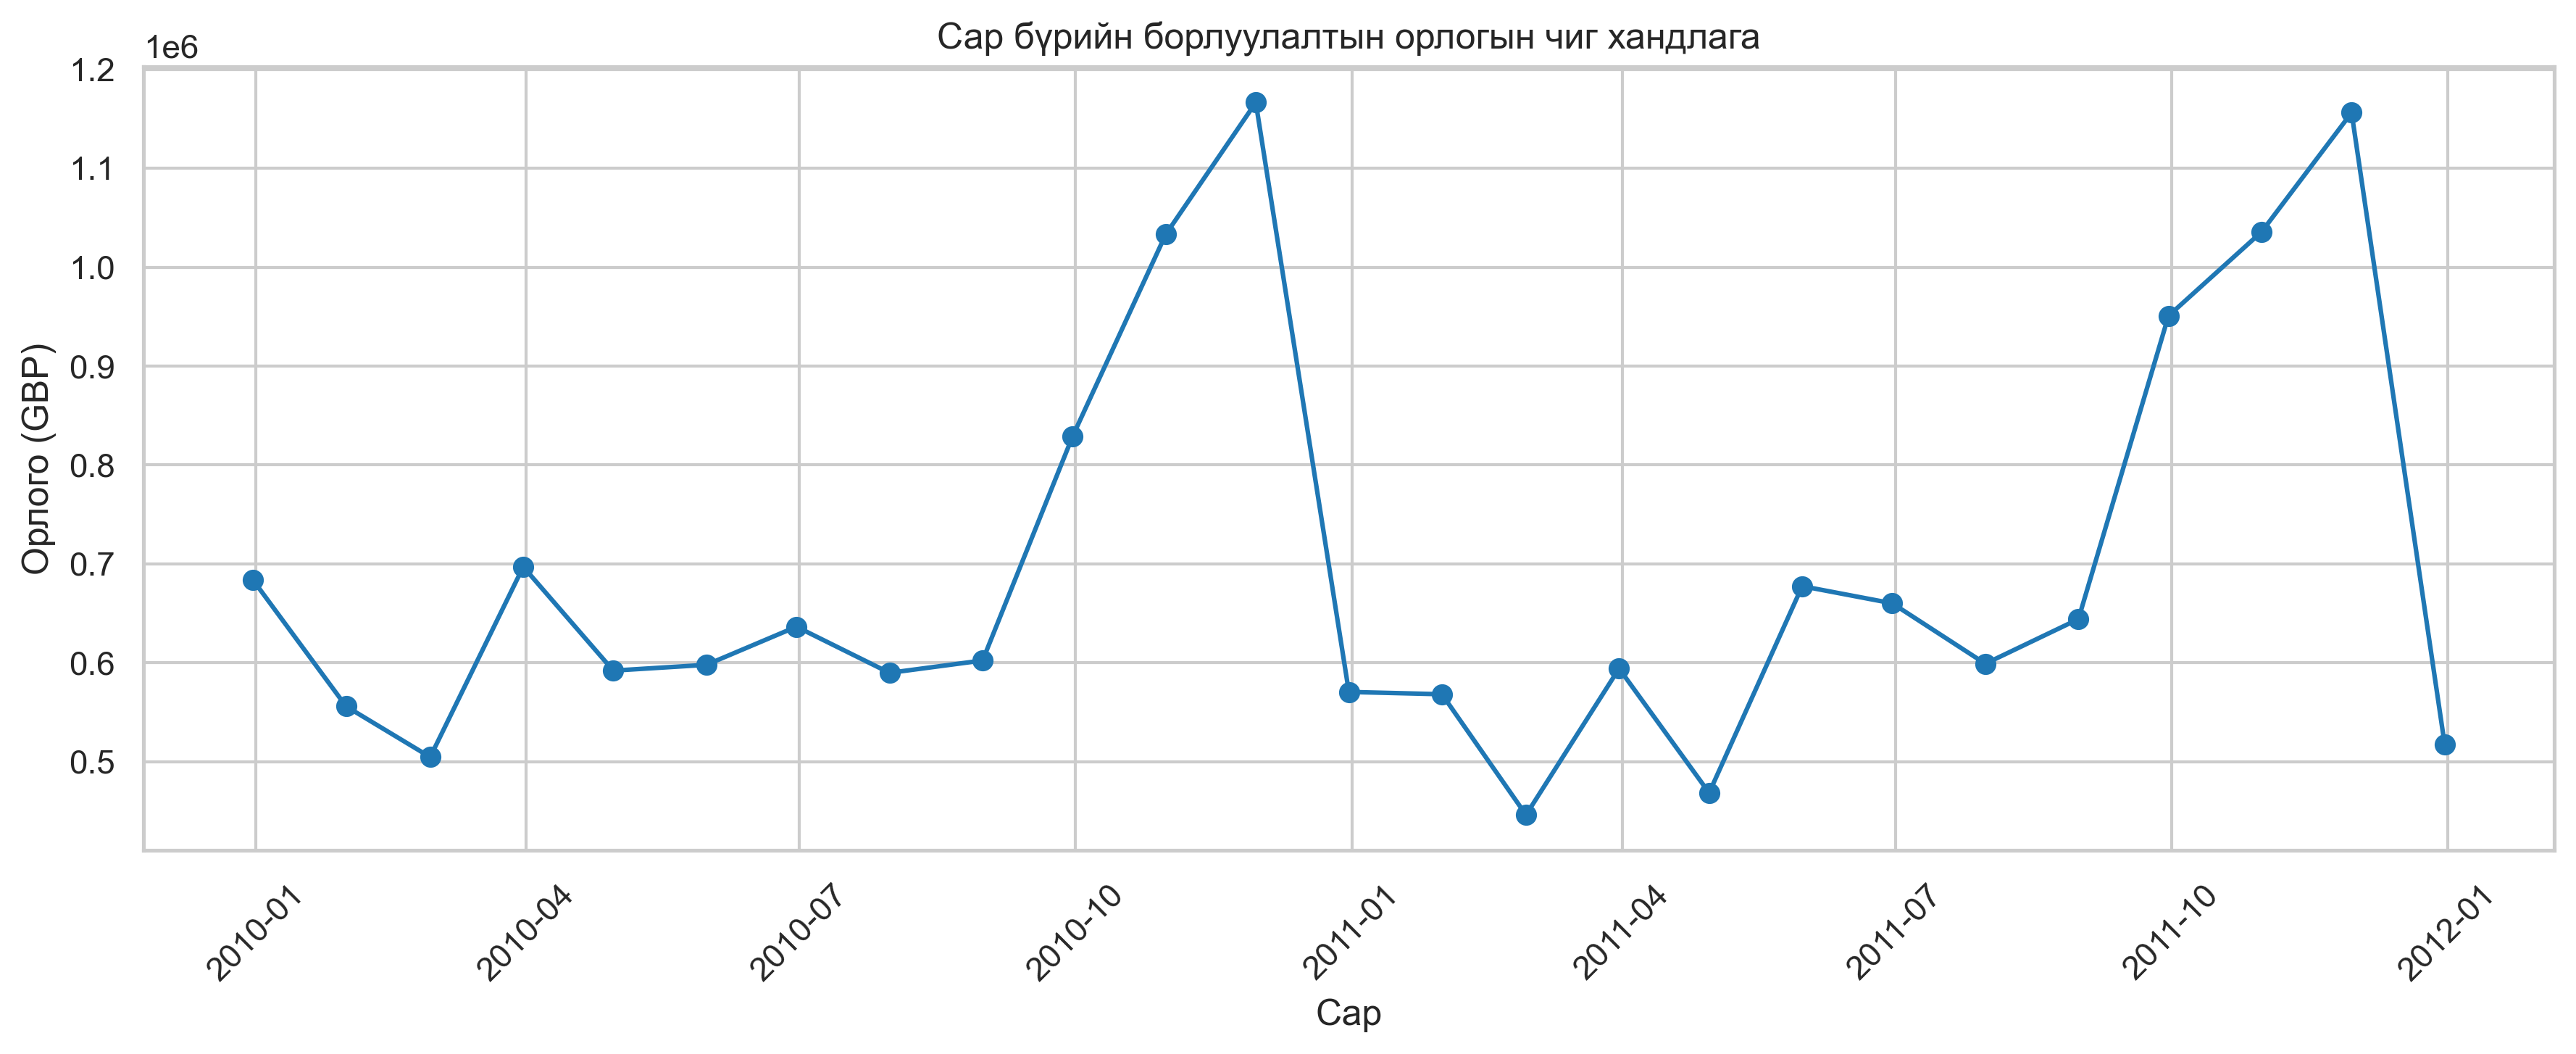
\includegraphics[width=0.85\textwidth]{monthly_revenue.png}
    \caption{\small 2010--2011 оны сар бүрийн орлого}
\end{figure}
\small
\begin{itemize}
    \item 9--12 саруудад оргил хүрч 1-р сард бууралт
    \item Улирлын хэв шинж тод илэрч байна
\end{itemize}
\end{frame}

\begin{frame}{Орлогоор тэргүүлэгч бүтээгдэхүүн}
\begin{figure}
    \centering
    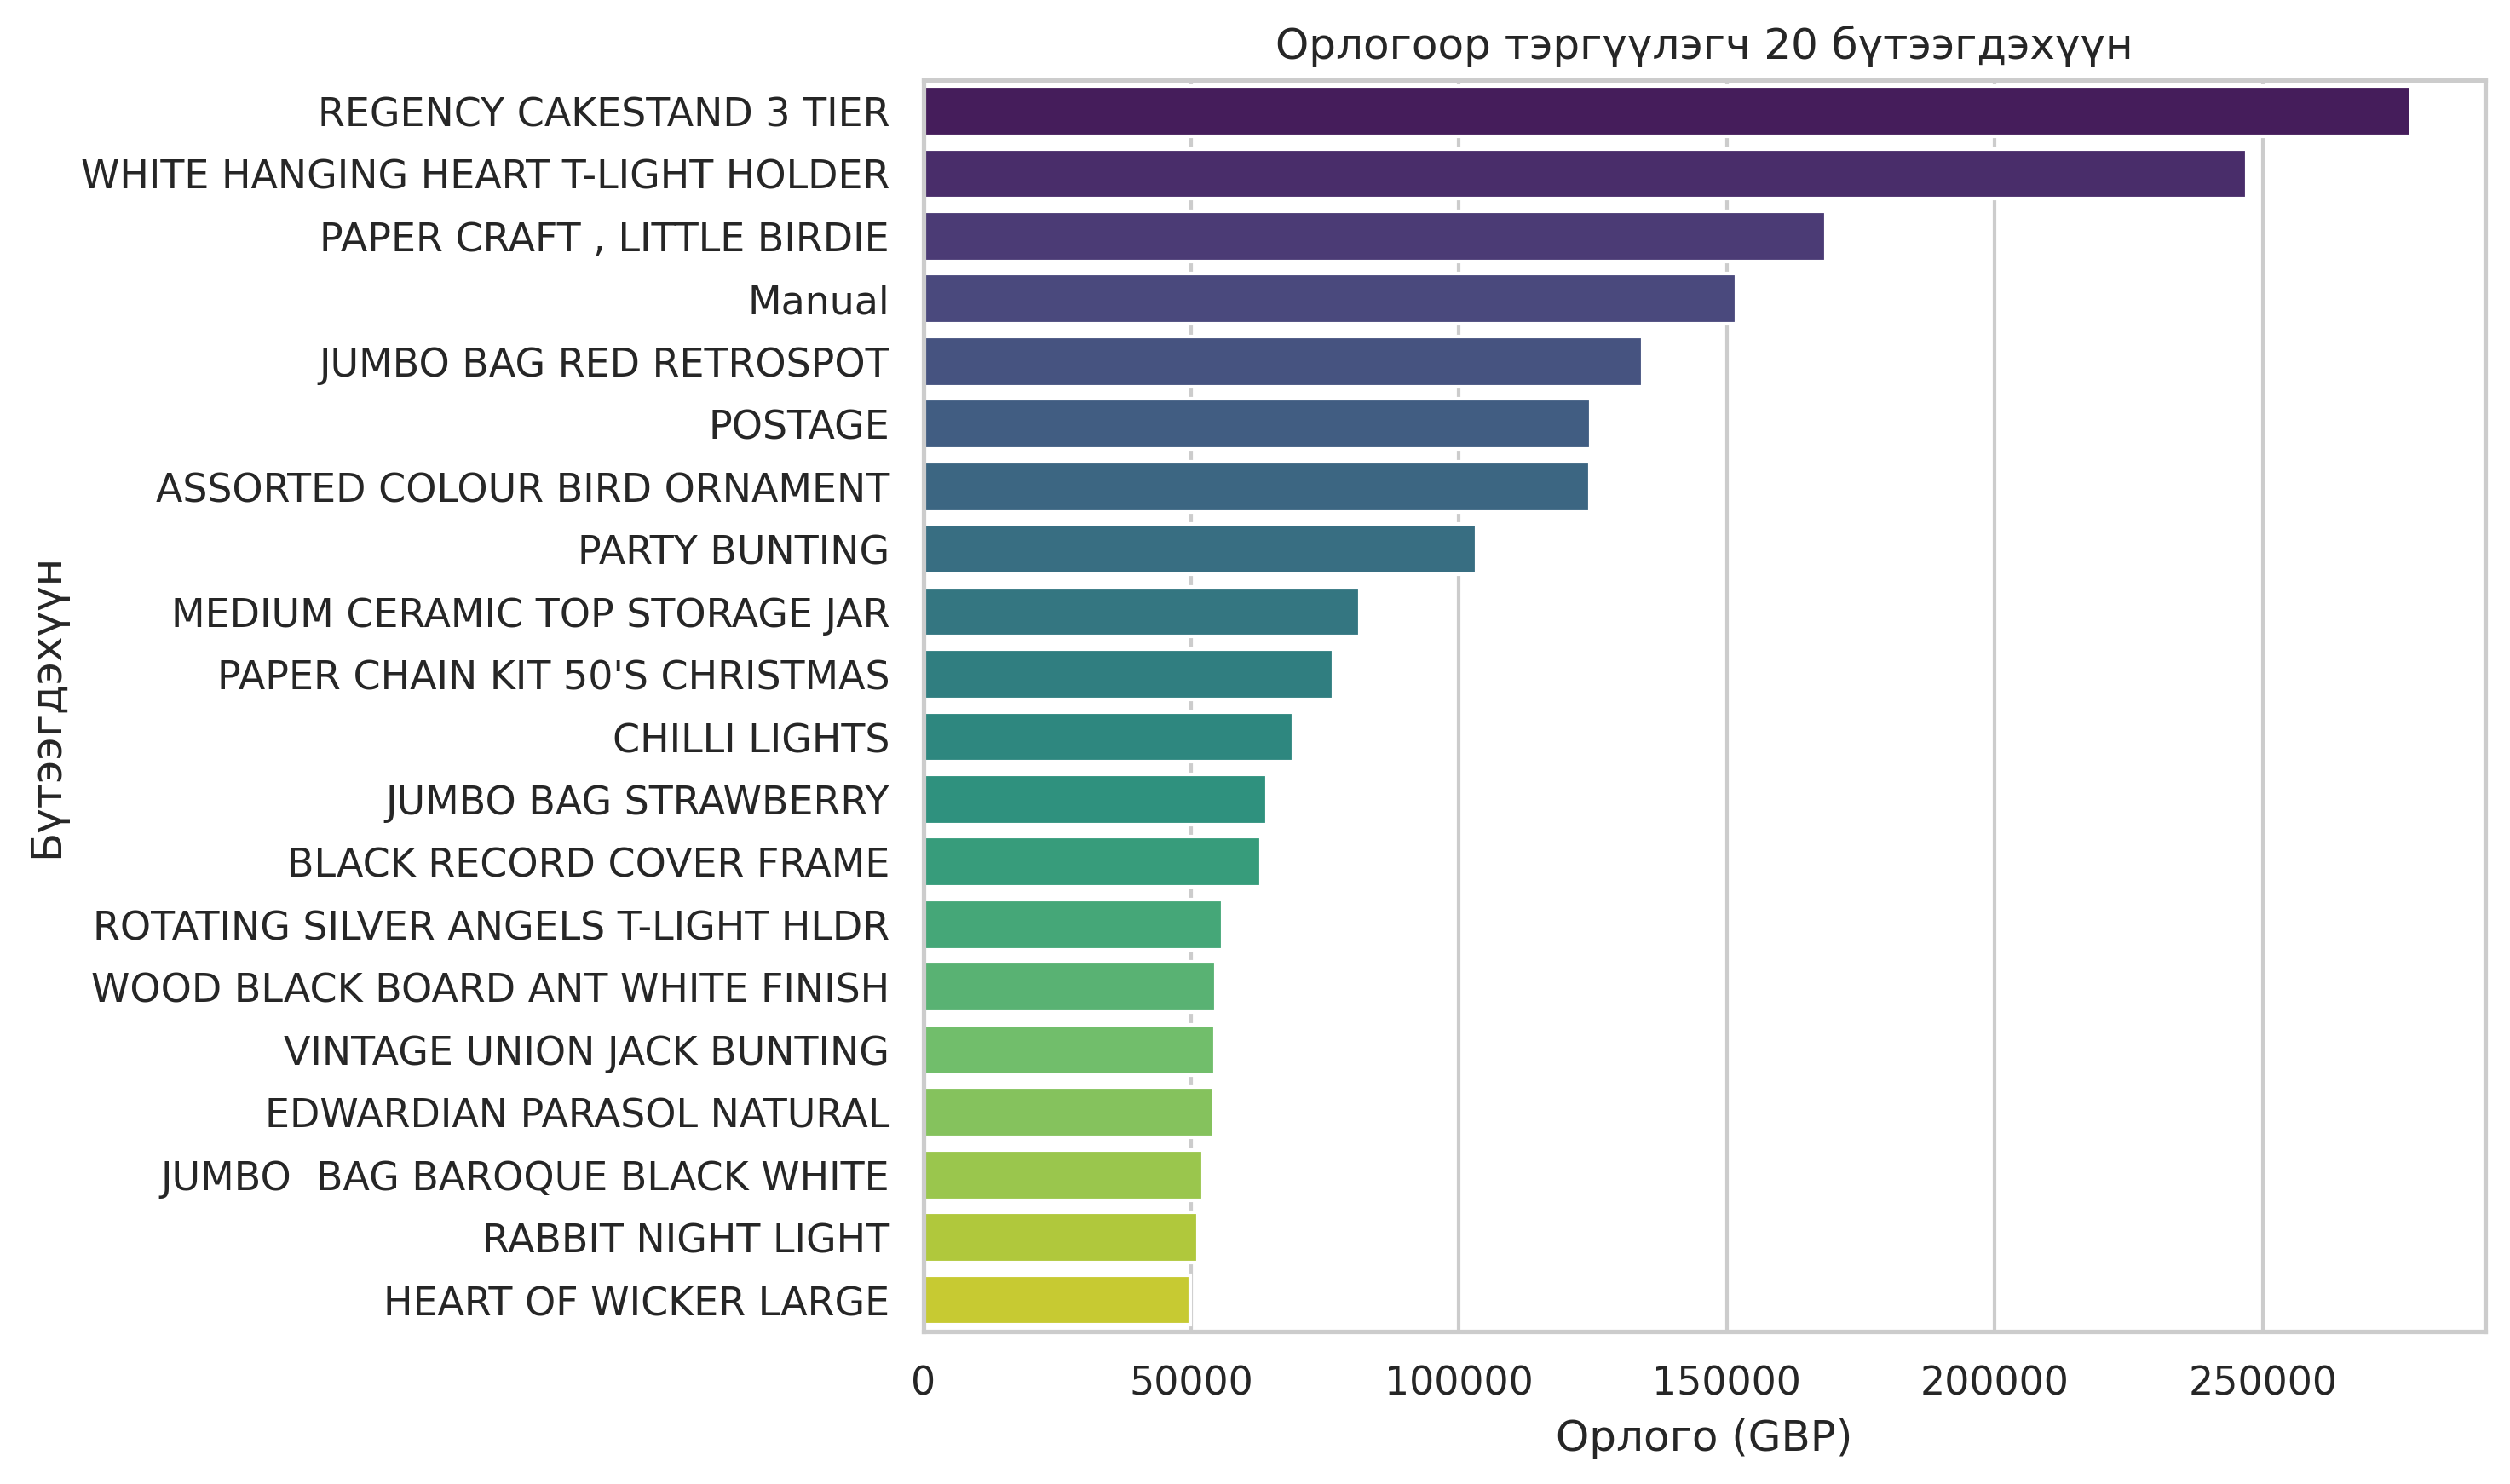
\includegraphics[width=0.9\textwidth]{top_products_revenue.png}
    \caption{Топ 20 бүтээгдэхүүн}
\end{figure}
\end{frame}

\begin{frame}{Орлогоор тэргүүлэгч улсууд}
\begin{figure}
    \centering
    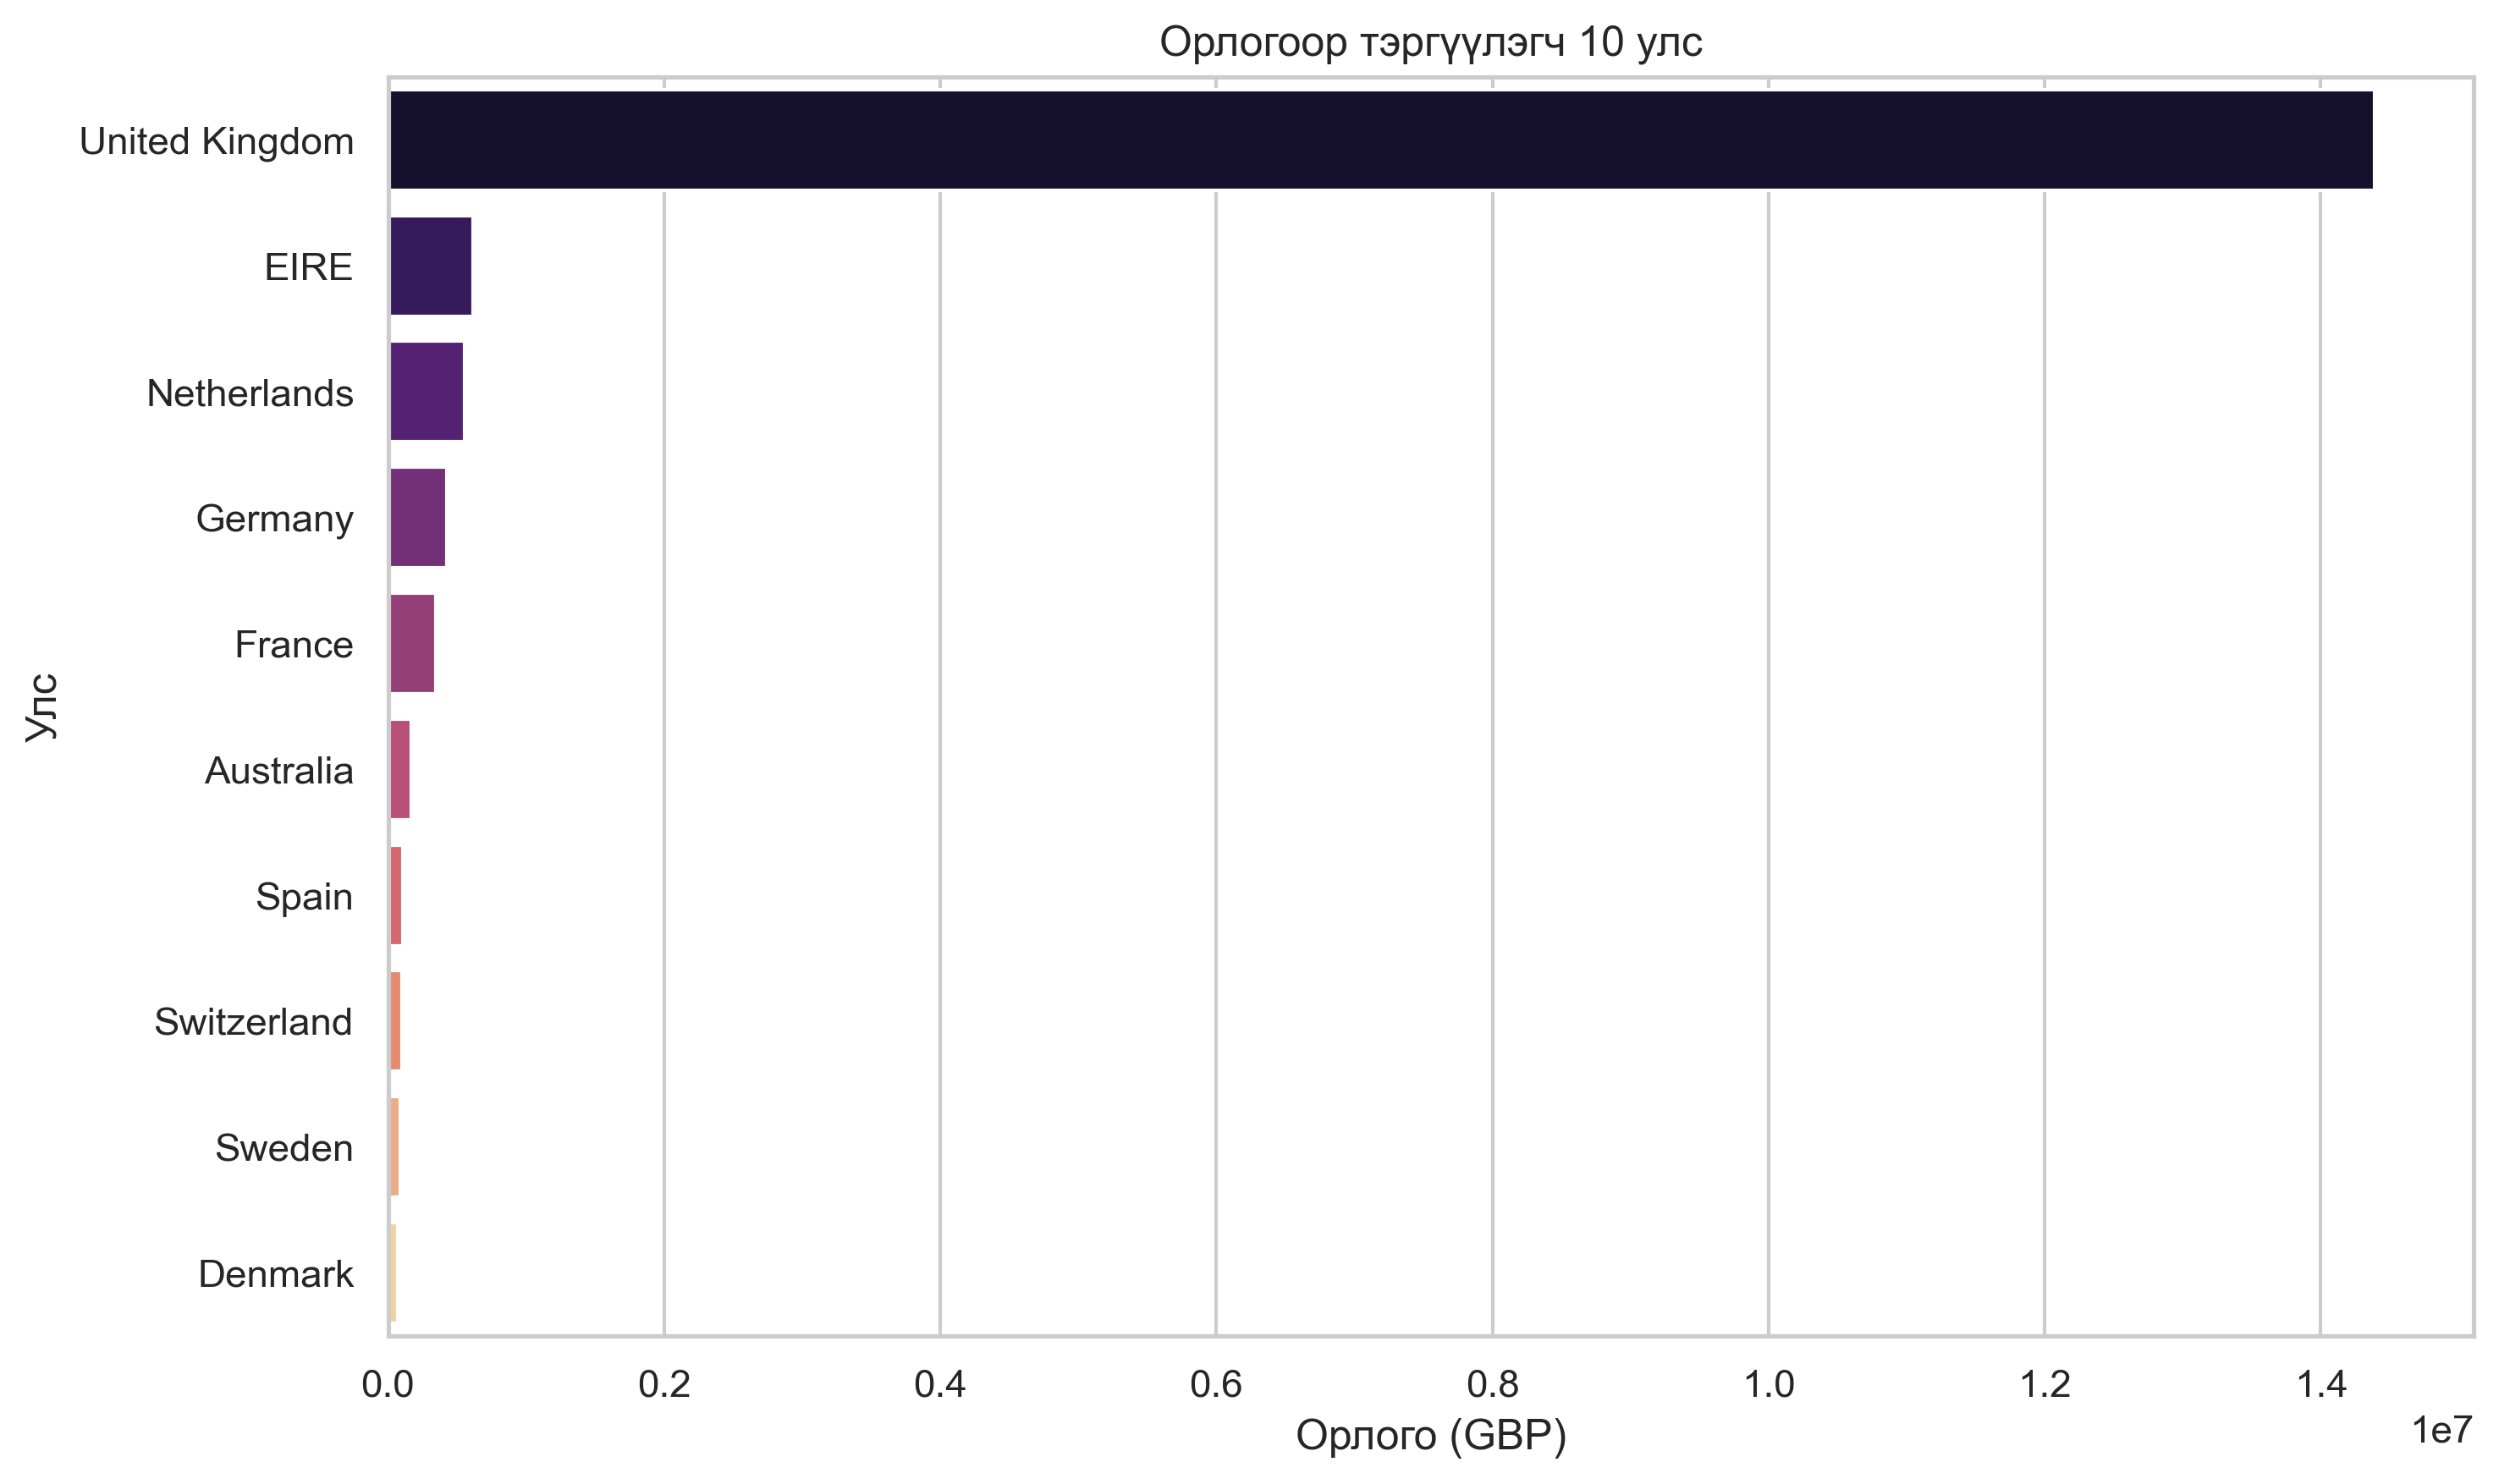
\includegraphics[width=0.9\textwidth]{top_countries_revenue.png}
    \caption{Топ 10 улс}
\end{figure}
\end{frame}

\begin{frame}{RFM шинжилгээ}
\begin{figure}
    \centering
    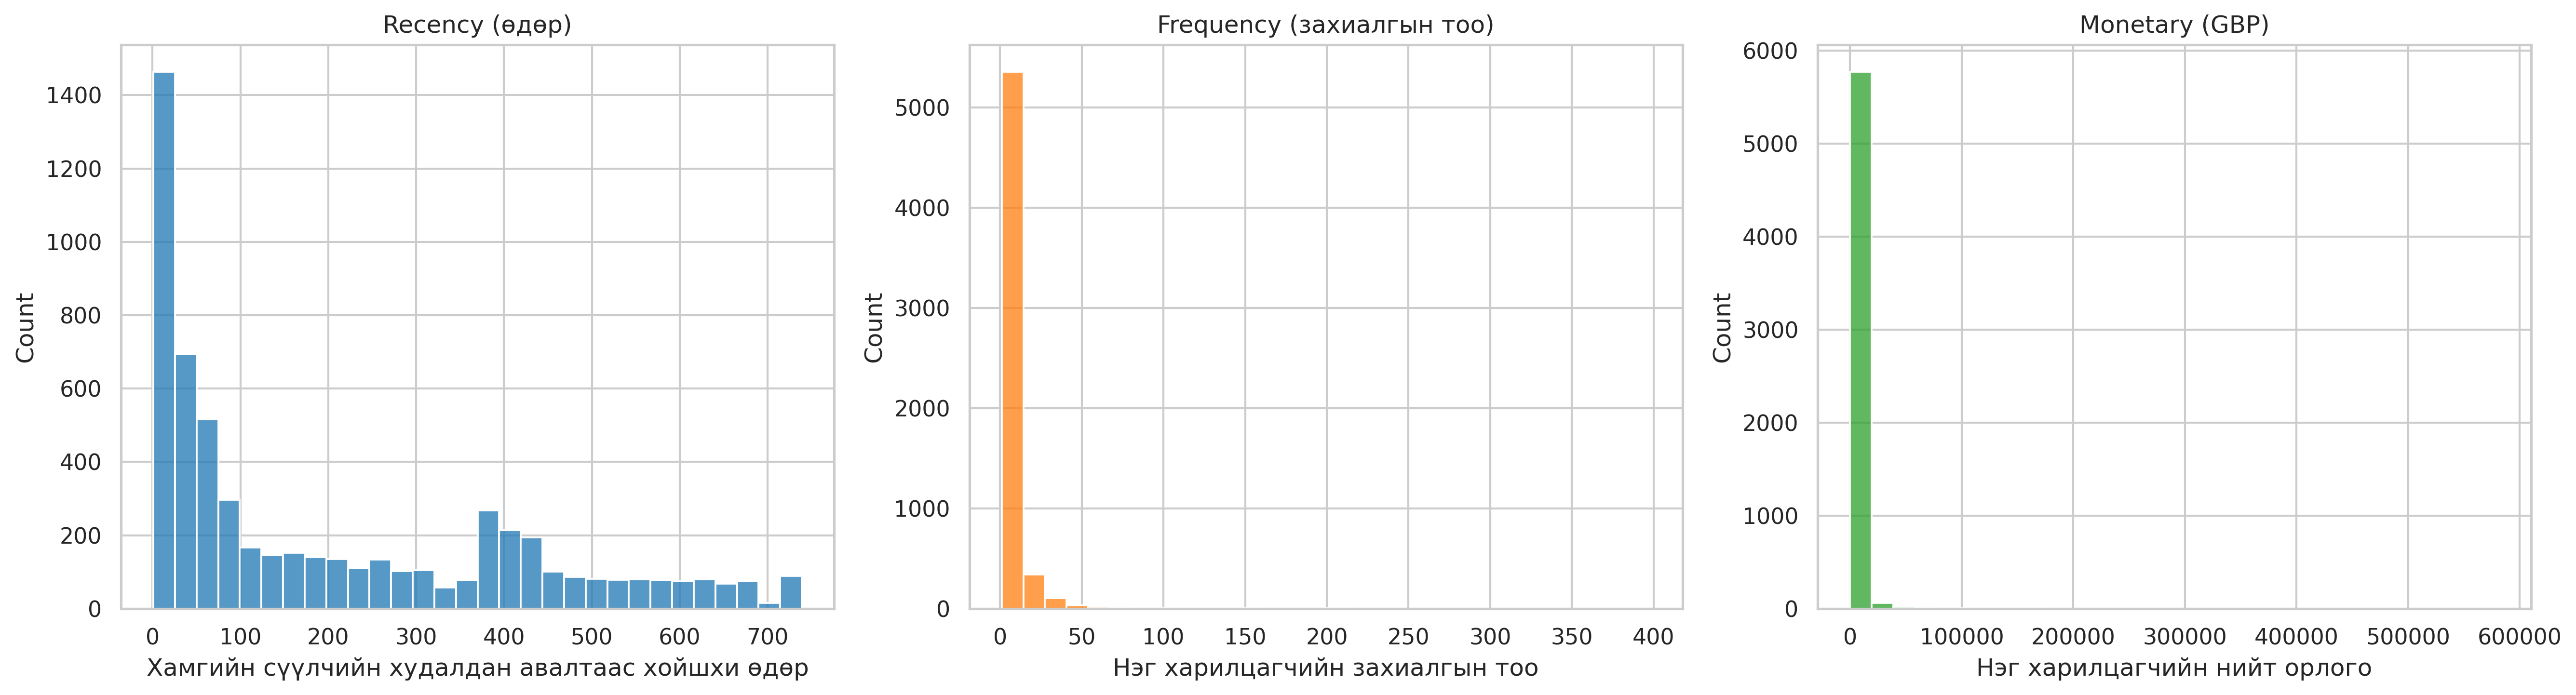
\includegraphics[width=0.95\textwidth]{rfm_distribution.png}
    \caption{Recency, Frequency, Monetary тархалт}
\end{figure}
\end{frame}

\begin{frame}{RFM дүн шинжилгээ}
\small
\textbf{Гол ажиглалтууд:}
\begin{itemize}
    \item Recency 0--7 хоногтой ~300 харилцагч\\орлогын \textbf{25\%}-ийг бүрдүүлнэ
    \item Frequency ≥ 10 бүхий харилцагчид\\дундаж орлогоороо \textbf{5 дахин} өндөр
    \item RFM оноо 10+ сегмент: \textbf{1,100} VIP
    \item RFM оноо ≤ 5: \textbf{2,200} идэвхжүүлэх хэрэгтэй
\end{itemize}

\vspace{0.2cm}
\textbf{Бизнесийн зөвлөмж:}
\begin{itemize}
    \item VIP: лояалти хөтөлбөр
    \item Идэвхгүй: сэргээх кампани
\end{itemize}
\end{frame}

\section{Churn загварчлал}

\begin{frame}{Churn тодорхойлолт}
\small
\textbf{Онолын хүрээ:}
\begin{itemize}
    \item Сүүлийн худалдан авалтаас хойш\\\textbf{90 хоног} захиалга хийхгүй бол churn
    \item Таслах огноо: \textbf{2011-09-10}
    \item Шошго тооцох: 2011-09-10 -- 2011-12-09
    \item 2 жилийн түүхэн өгөгдлөөс шинж үүсгэх
\end{itemize}

\vspace{0.2cm}
\textbf{Шинж чанарууд:}
\begin{itemize}
    \item Recency (хоногоор)
    \item Frequency (захиалгын тоо)
    \item Monetary (нийт орлого)
    \item Ялгаатай бүтээгдэхүүний тоо
\end{itemize}
\end{frame}

\begin{frame}{Загварын гүйцэтгэл}
\small
\textbf{Random Forest загвар:}
\begin{itemize}
    \item n\_estimators=200, class\_weight=balanced
    \item Train/test split: 75/25
\end{itemize}

\vspace{0.2cm}

\begin{tabularx}{\textwidth}{l>{\raggedleft\arraybackslash}X}
    \toprule
    Үзүүлэлт & Утга \\
    \midrule
    Accuracy & 0.708 \\
    F1-score & 0.648 \\
    ROC-AUC & 0.773 \\
    True Positive & 355 \\
    False Negative & 218 \\
    False Positive & 168 \\
    True Negative & 580 \\
    \bottomrule
\end{tabularx}
\end{frame}

\begin{frame}{Churn загварын дүгнэлт}
\small
\textbf{Амжилт:}
\begin{itemize}
    \item ROC-AUC 0.773 нь сайн ялгах чадвар
    \item Дөрвөн энгийн шинжээр\\үр дүнтэй таамаглал
    \item Загварыг \texttt{churn\_model\_rf.pkl}\\хэлбэрээр хадгалсан
\end{itemize}

\vspace{0.2cm}
\textbf{Дараагийн алхам:}
\begin{itemize}
    \item Нэмэлт шинж: маркетинг суваг,\\үнийн уян хатан чанар
    \item Босго тохируулж recall нэмэх
    \item Бизнесийн өртгийн функц ашиглах
\end{itemize}
\end{frame}

\section{Таамаглал}

\begin{frame}{Топ 20 бүтээгдэхүүний орлогын цуваа}
\begin{figure}
    \centering
    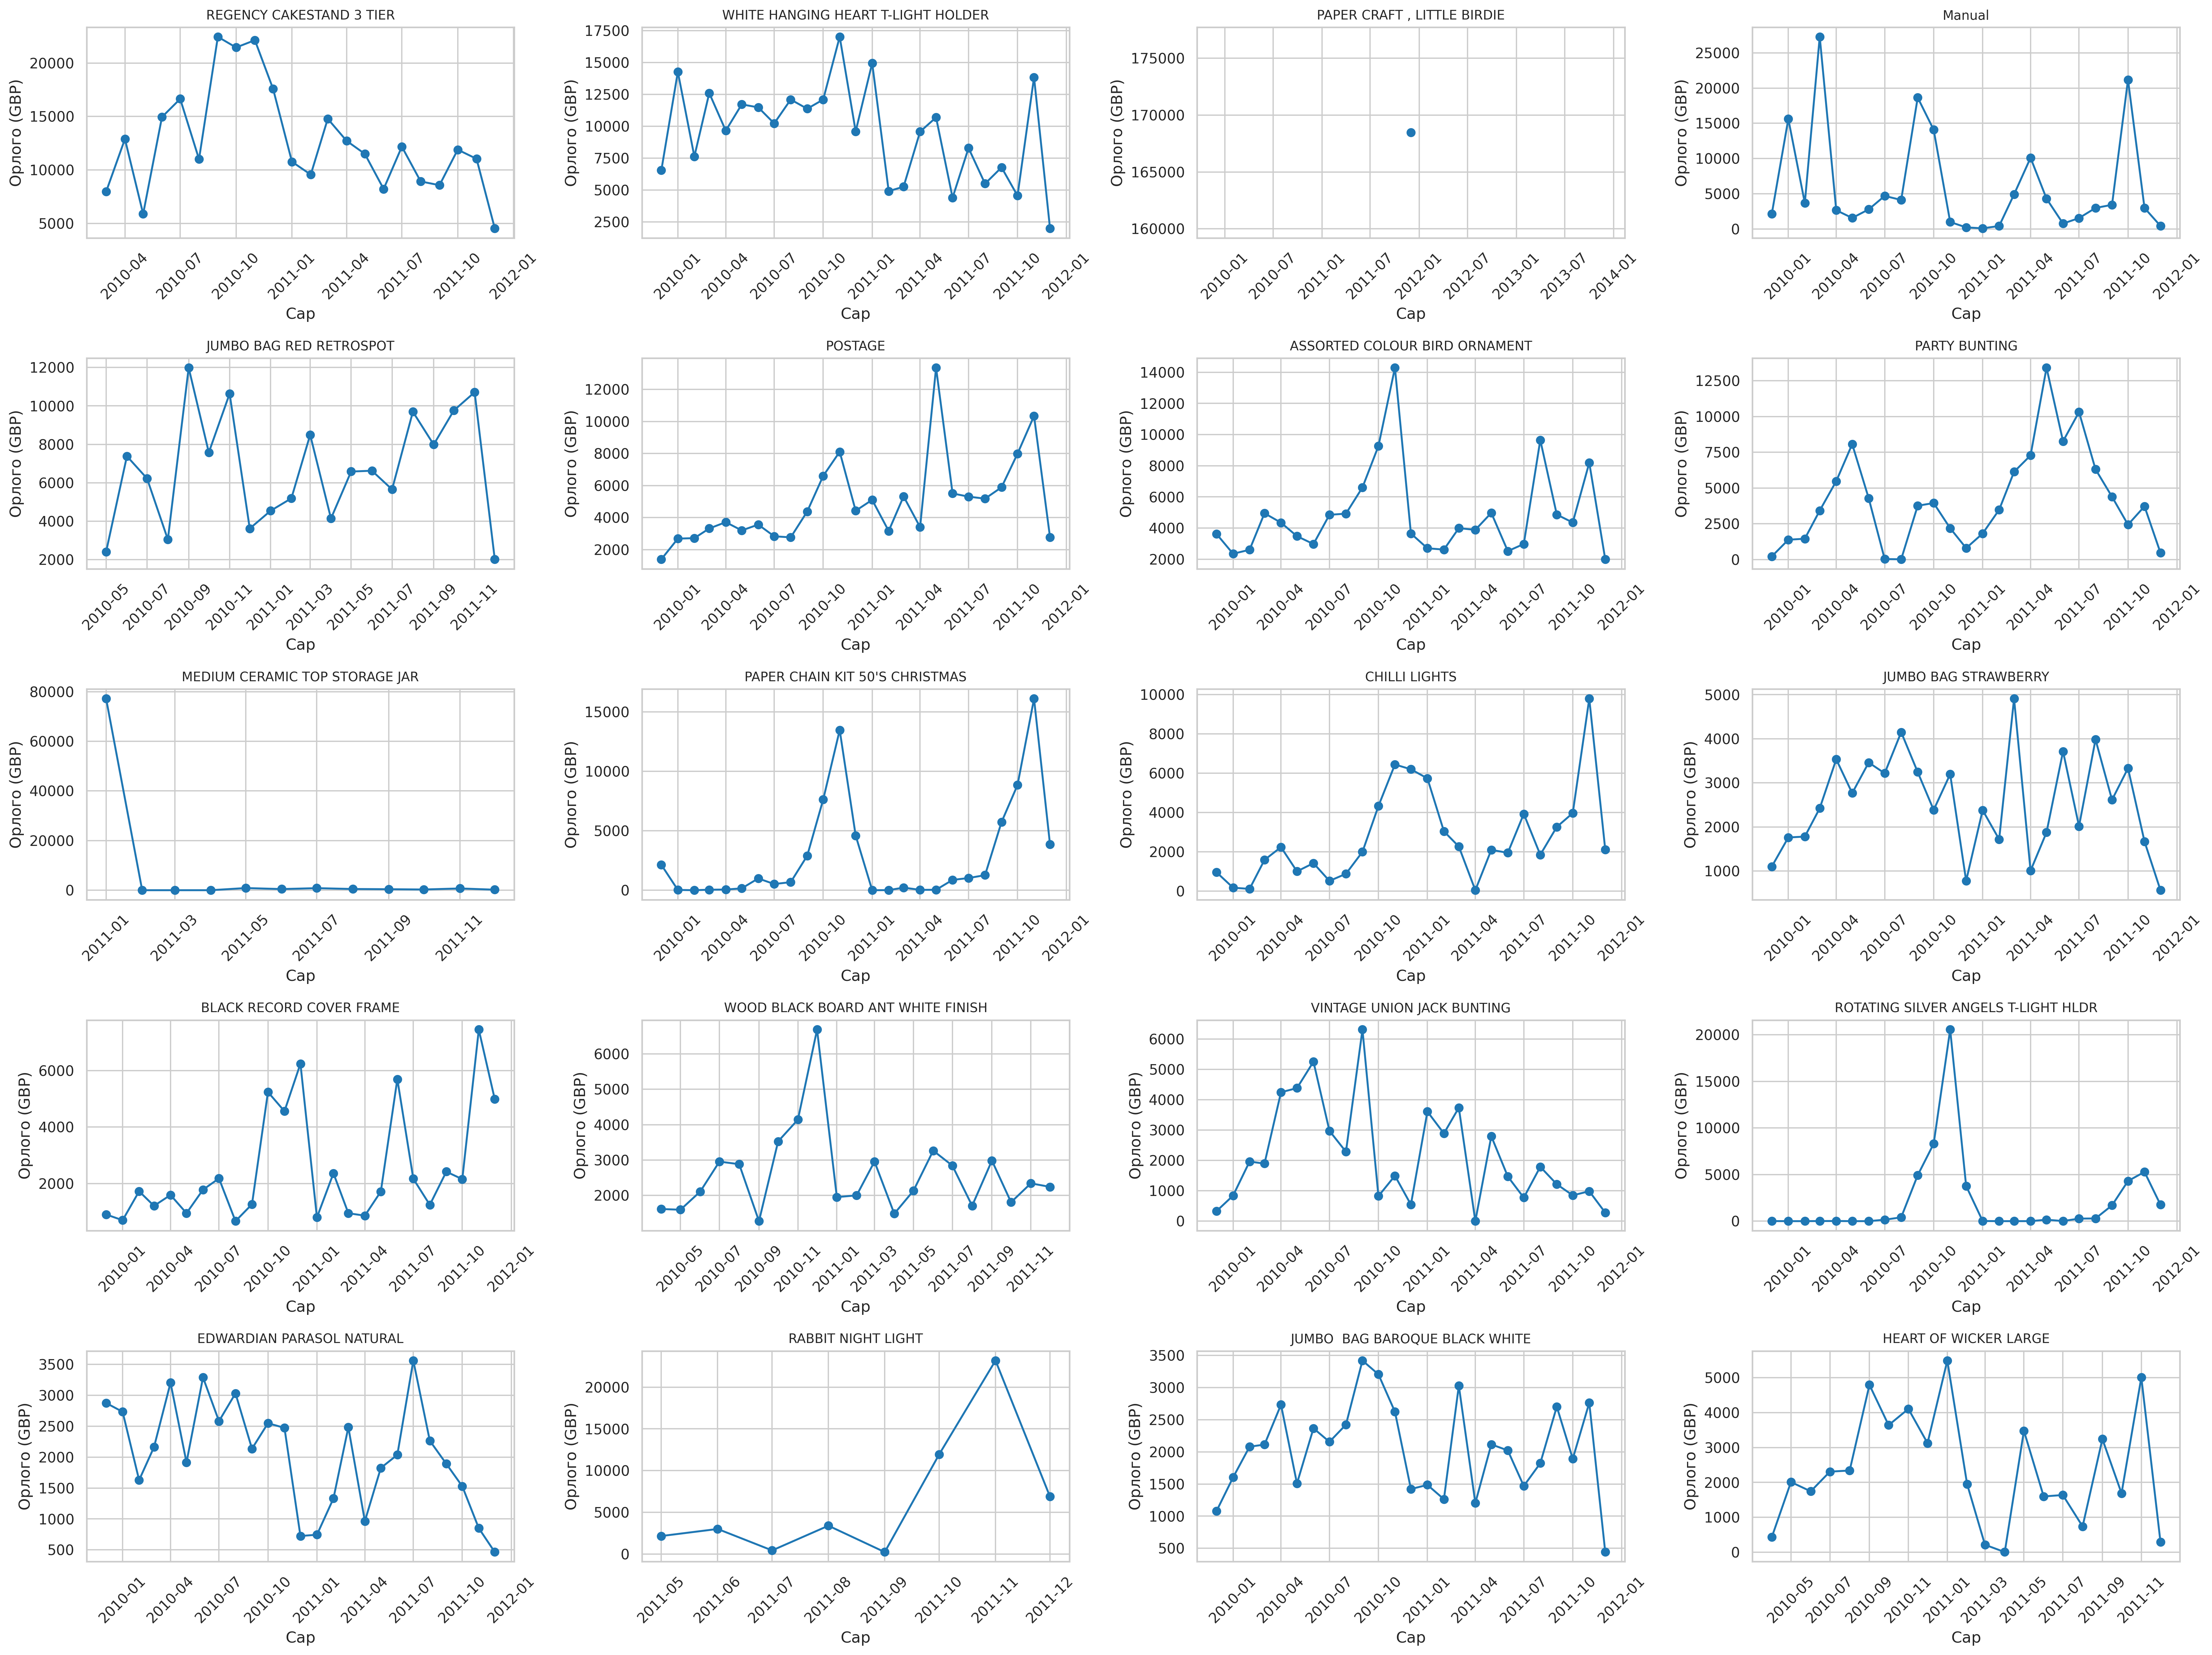
\includegraphics[width=0.9\textwidth]{top20_monthly_revenue_trends.png}
    \caption{Сүүлийн 24 сарын сар бүрийн орлого (топ 20)}
\end{figure}
\end{frame}

\begin{frame}{Таамаглалын загварууд}
\small
\textbf{Гурван загвар харьцуулах:}
\begin{enumerate}
    \item \textbf{Naive:} Сүүлийн утгыг хадгална
    \item \textbf{Exponential Smoothing:}\\Holt-ийн additive trend
    \item \textbf{ARIMA(1,1,1):} Автокорреляц загвар
\end{enumerate}

\vspace{0.2cm}
\textbf{Үнэлгээний арга:}
\begin{itemize}
    \item 3 сарын таамаглал
    \item SMAPE (Symmetric Mean Absolute\\Percentage Error)
    \item Walk-forward validation
\end{itemize}
\end{frame}

\begin{frame}{Таамаглалын харьцуулалт}
\begin{figure}
    \centering
    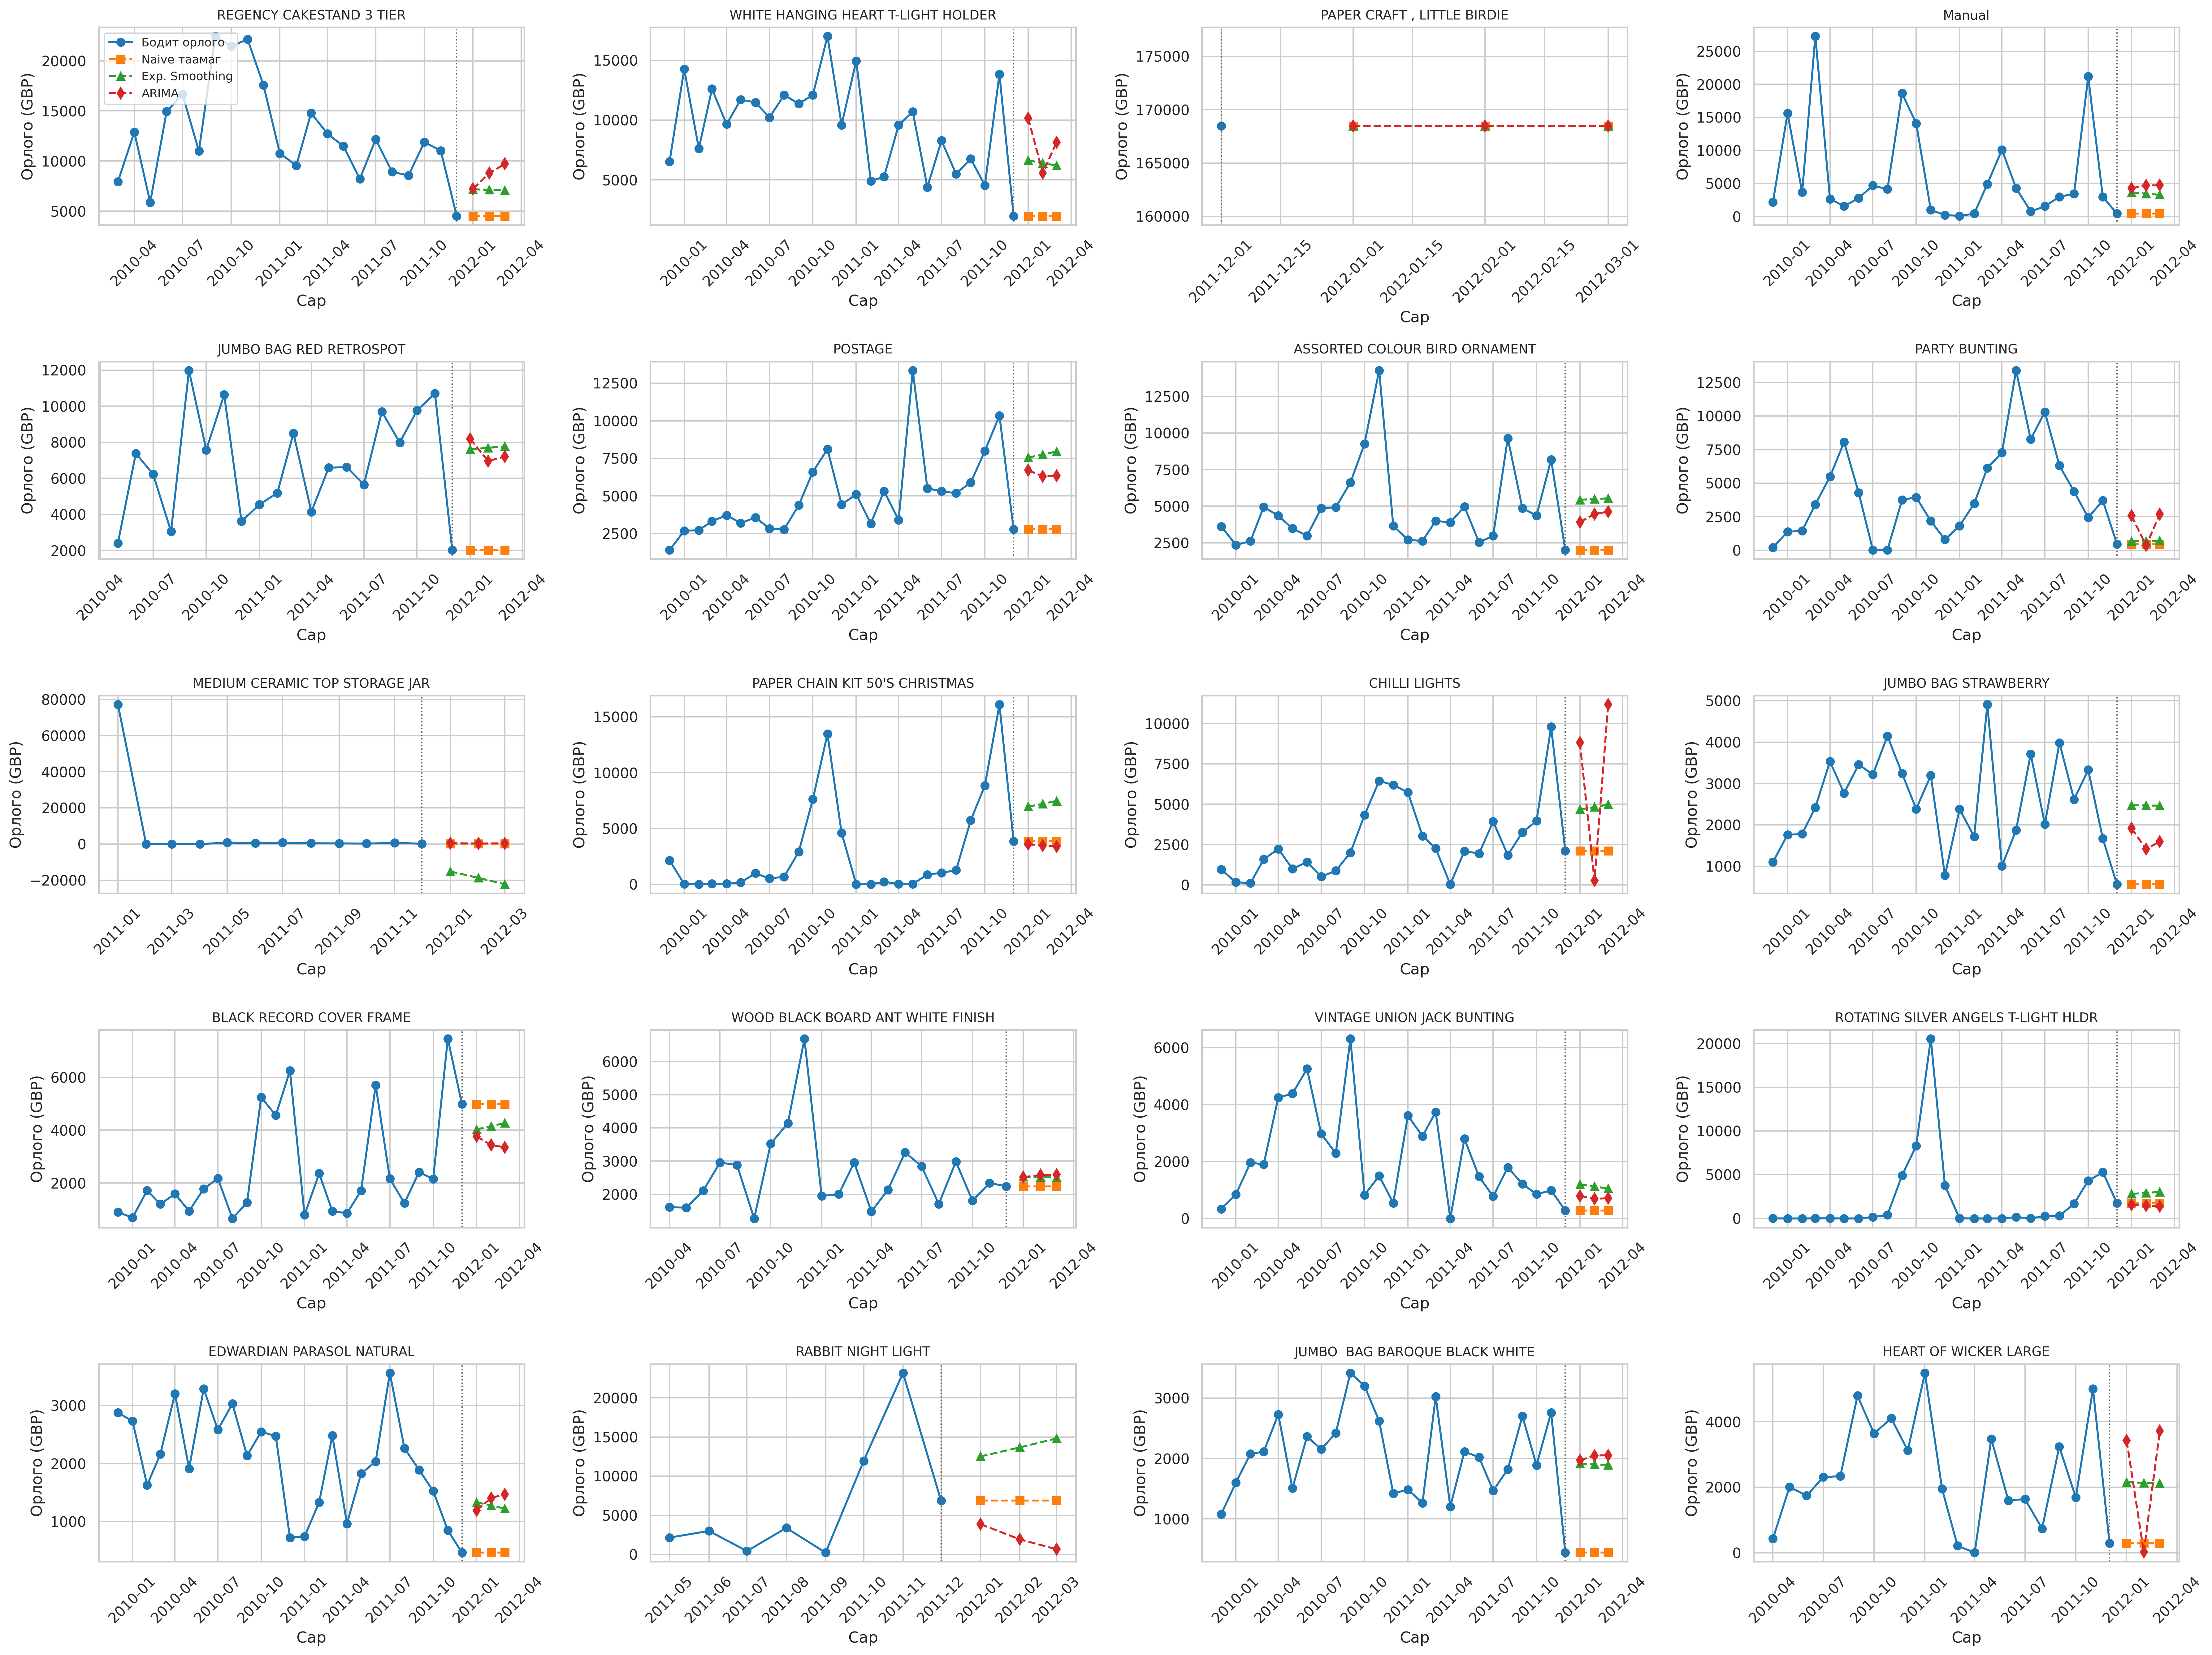
\includegraphics[width=0.9\textwidth]{top20_forecast_comparison.png}
    \caption{Naive, Exponential Smoothing, ARIMA загварын харьцуулалт}
\end{figure}
\end{frame}

\begin{frame}{SMAPE үр дүн}
\small
\begin{tabularx}{\textwidth}{l>{\raggedleft\arraybackslash}X>{\raggedleft\arraybackslash}X>{\raggedleft\arraybackslash}X}
    \toprule
    Загвар & Дундаж & Медиан & Давуу \\
    \midrule
    Naive & 69.35 & 60.44 & 6 \\
    Exp. Smoothing & 72.26 & 60.59 & 7 \\
    ARIMA(1,1,1) & 67.10 & 59.96 & 6 \\
    \bottomrule
\end{tabularx}

\vspace{0.2cm}
\textbf{Гол ажиглалт:}
\begin{itemize}
    \item ARIMA дундаж SMAPE хамгийн бага (67.1)
    \item Улирлын оргилтой бүтээгдэхүүнд\\ES илүү сайн
    \item Богино цуваанд загварууд ойролцоо
\end{itemize}
\end{frame}

\begin{frame}{Загварын харьцуулалт}
\small
\textbf{Гүйцэтгэлийн шинжилгээ:}
\begin{itemize}
    \item ARIMA дундаж SMAPE 67.1-тай\\хамгийн сайн гүйцэтгэл
    \item Naive 69.35, ES 72.26 SMAPE
    \item Цуваа 12--24 ажиглалтаас бүрдэх\\(хэт богино түүх)
    \item Загварууд давуу тал ижил (6-6-7)
\end{itemize}

\vspace{0.2cm}
\textbf{Санал:}
\begin{itemize}
    \item SARIMA (улирлын параметртэй) турших
    \item Экзоген хувьсагч (кампани,\\өдрийн төрөл) нэмэх
    \item Илүү урт түүхэн өгөгдөл цуглуулах
\end{itemize}
\end{frame}

\section{Дүгнэлт}

\begin{frame}{Гол сургамж}
\small
\begin{enumerate}
    \item \textbf{Өгөгдөл:} 779k+ мөр, £17.4M орлого,\\найдвартай суурь
    \item \textbf{EDA \& RFM:} VIP сегмент орлогын\\25\%-ийг бүрдүүлдэг; улирлын оргил Q4-т
    \item \textbf{Churn:} ROC-AUC 0.773, дөрвөн шинжээр\\эрсдэлтэй сегмент илрүүлэх
    \item \textbf{Таамаглал:} ARIMA дундаж сайн;\\улирлын бүтээгдэхүүнд ES давуу
\end{enumerate}
\end{frame}

\begin{frame}{Бизнесийн зөвлөмж}
\small
\textbf{Харилцагчийн менежмент:}
\begin{itemize}
    \item VIP сегмент (RFM ≥ 10):\\лояалти хөтөлбөр, VIP урамшуулал
    \item Идэвхгүй сегмент (RFM ≤ 5):\\имэйл, купон, ремаркетинг
\end{itemize}

\vspace{0.2cm}
\textbf{Борлуулалтын төлөвлөлт:}
\begin{itemize}
    \item Q4-н өмнө нөөц нэмэгдүүлэх\\(баярын улирал)
    \item Cross-sell, bundle санал\\(бэлгийн багц + гэр ахуй)
    \item UK дотор сегментчилэх,\\Европ руу өргөжүүлэх
\end{itemize}
\end{frame}

\begin{frame}{Дараагийн алхам}
\small
\textbf{Техникийн сайжруулалт:}
\begin{itemize}
    \item Churn: маркетинг суваг,\\үнийн мэдрэмж нэмэх
    \item Forecast: SARIMA,\\экзоген хувьсагчтай модель
    \item A/B тест: кампанит ажлын\\үр дүнг хэмжих
\end{itemize}

\vspace{0.2cm}
\textbf{Хэрэгжүүлэлт:}
\begin{itemize}
    \item Загварыг API болгон\\үйлдвэрлэлд нэвтрүүлэх
    \item Автомат тайлан (сар бүр)\\үүсгэх систем
    \item Шинэ өгөгдлөөр загварыг\\дахин сургах процесс
\end{itemize}
\end{frame}

\begin{frame}{Нэмэлт материал}
\small
\textbf{Гаралтын файлууд:}
\begin{itemize}
    \item \texttt{online\_retail\_cleaned.csv}\\цэвэр өгөгдөл
    \item \texttt{churn\_model\_rf.pkl}\\сургасан загвар
    \item \texttt{forecast\_evaluation\_top20.csv}\\SMAPE үр дүн
    \item \texttt{top20\_forecasts\_next3months.csv}\\таамаглал
\end{itemize}

\vspace{0.2cm}
\textbf{Код:}
\begin{itemize}
    \item \texttt{mcs\_task.ipynb}\\иж бүрэн шинжилгээ
    \item Бүх график: \texttt{figures/} фолдер
\end{itemize}
\end{frame}

\begin{frame}
\centering
\Huge Баярлалаа!

\vspace{1cm}

\Large Асуулт байна уу?
\end{frame}

\end{document}
